\section[Contexte des langages dédiés s'appliquant aux ordonnanceurs d'E/S sous Linux (A CHANGER)]{Contexte des langages dédiés s'appliquant aux or-donnanceurs d'E/S sous Linux (A CHANGER)}
\label{context}

\subsection{Les planificateurs d'E/S}

Dans leur fonctionnement, les ordonnanceurs de lecture (sortie) et d'écriture 
(entrée) tentent d'améliorer le débit en réorganisant l'accès aux requêtes dans 
un ordre linéaire basé sur les adresses logiques des données sur le disque, en 
essayant de les fusionner. Bien que cela puisse augmenter le débit global, 
certaines requêtes d'E/S peuvent attendre trop longtemps, provoquant des 
problèmes de latence et des fois de famine. Les planificateurs d'E/S tentent 
d'équilibrer le besoin d'un débit élevé tout en essayant de partager 
équitablement les requêtes d'E/S entre les processus.

Différentes approches ont été adoptées pour divers planificateurs d'E/S et 
chacun a ses propres forces et faiblesses et de manière générale, il n'y a pas 
de planificateur d'E/S par défaut parfait pour toute la gamme de requêtes d'E/S 
qu'un système peut rencontrer. 

\subsection{État de l'art}

Historiquement, les premiers algorithmes d'ordonnancement qui ont été 
développés se sont basés sur la structure interne des disques durs de l'époque, 
que l'on retrouve aujourd'hui encore dans beaucoup d'ordinateur. Cette 
structure organisée par secteurs de données sur plateaux était lue par une tête 
de lecture unique, limitant ainsi les actions possibles sur le disque à une 
seule écriture ou une seule lecture à la fois. Les algorithmes de l'époque ont 
donc étaient développés en conséquence, et sont devenus au fur et à mesure du 
temps obsolètes. La sortie de nouvelles technologies à la mémoire flash, comme 
les disques SSD (Solid-State Drive) ont offert la possibilité de pouvoir 
effectuer plusieurs lectures et plusieurs écritures de manière simultanée. Ces 
nouvelles technologies ont donc donnée naissance à de nouveaux algorithmes, 
comme BFQ en 2003, ou Kyber, développé en 2017 par Facebook.

Aujourd'hui dans Linux il existe plusieurs ordonnanceurs, tous ayant une 
utilité situationnelle et de manière générale, ils se distinguent entre deux 
catégories. Première-ment il y a les ordonnanceurs à file d'attente simple, ce 
sont les premiers qui ont existé et qui sont maintenant dépréciés dans les 
versions de Linux actuelles (depuis la version 5.3). Puis il y a les 
ordonnanceurs à file d'attente multiples, leur tâche est de distribuer les 
requêtes d'E/S aux différents fils d'exécution du noyau qui seront ensuite 
distribués aux différents processeurs. Voici une liste exhaustive des 
planificateurs existant dans Linux :

\begin{center}
    \begin{tabularx}{\textwidth} { 
        | >{\hsize=0.22\hsize\linewidth=\hsize\raggedright\arraybackslash}X 
        | >{\hsize=0.23\hsize\linewidth=\hsize\raggedright\arraybackslash}X 
        | >{\hsize=1.55\hsize\linewidth=\hsize\arraybackslash}X | }
        \hline
        Nom & Catégorie de file d'attente & Description \\
        \hline
        \hline
        Deadline & Simple & Conçu pour régler les problèmes de famine aperçu 
        dans d'autres ordonnanceurs à l'époque. Son algorithme utilise 3 files, 
        à savoir une file dite ``triée'' (par priorité), une file de lecture et 
        une file d'écriture. Les requêtes de la file triée sont prioritaires et 
        si une des requêtes des deux autres files expire, elle devient 
        prioritaire. Les lectures ont un délai d'expiration de 0.5s par défaut 
        tandis que les écritures sont moins privilégiées avec 5s d'expiration. 
        \\
        \hline
        CFQ & Simple & Conçu pour se rapprocher des processus. Possède des 
        files distinctes par processus et se base sur la valeur ``ionice'' pour 
        les priorités. Chaque file se voit attribuer un temps d'équité, pouvant 
        provoquer ainsi des situation de ``vide'' si le temps attribué n'est 
        pas utilisé. \\
        \hline
        Noop & Simple & Aucun tri n'est effectué avec cet algorithme 
        d'ordonnancement, seulement des fusions de requêtes aux adresses 
        voisines. Il peut être efficace dans de rare cas, mais cela inclu les 
        contrôleurs de stockage avancés, qui trient eux-même leur requêtes \\
        \hline
        BFQ (Budget Fair Queuing) & Multiple & Conçu pour fournir une bonne 
        réponse interactive, en particulier pour les périphériques d'E/S lents. 
        Il n'est cependant pas idéal pour les périphériques dotés de 
        processeurs lents car chaque opération entraine une surchage de travail 
        assez élévée. La notion d'équité ici repose sur la taille des données 
        demandées plutôt que sur le temps. \\
        \hline
        Kyber & Multiple & Créé pour les périphériques multi-files rapides 
        comme les disques SSD ou les cartes \texttt{M.2} par exemple. Il reste 
        relativement simple et distribue les requêtes dans deux files : celle 
        des lectures et celle des écritures. Grâce à sa limitation du nombre de 
        requêtes pouvant être traitées à la fois, Kyber offre un temps de 
        service rapide pour les requêtes à haute priorités \cite{Kyber}. Il 
        sera souvent retrouvé comme ordonnanceur pour des serveurs, cependant 
        pour des machines avec un processeur plus lent, on retrouvera BFQ ou 
        MQ-Deadline. \\
        \hline
        None & Multiple & C'est tout simplement l'ordonnanceur qui n'en est pas 
        un. Aucune réorganisation des requêtes n'est effectuée, procurant ainsi 
        une surcharge minimale. Il peut être utile pour certains appareils très 
        rapides utilisant les technologies NVMe, comme les disques SSD. \\
        \hline
        MQ-Deadline & Multiple & C'est la version multi-files de l'algorithme 
        ``Deadline'', polyvalent, il reste le plus souvent utilisé dû à sa 
        faible surcharge CPU.\\
        \hline
    \end{tabularx}
\end{center}

\vspace{5mm}

Tout ces ordonnanceurs présentés précédemment ont cependant tous un point 
commun, ils sont écris à la main par un développeur du noyau Linux. Le projet 
VeriAMOS essaye de changer cet aspect en proposant au développeur n'ayant pas 
toute la connaissance du noyau linux de pouvoir créer son propre planificateur 
facilement grâce à PhaistOS. 

\subsection{Arborescence du projet}

PhaistOS est un DSL comme nous l'avons compris, il a été développé par Nick 
Papoulias (ancien membre de l'équipe Erods) comme sujet de post doctorat. Il 
s'est attelé au développement de PhaistOS avec le langage de programmation 
Ocaml et a organisé l'architecture du DSL de la sorte :

\begin{figure}[h!t] \centering
    %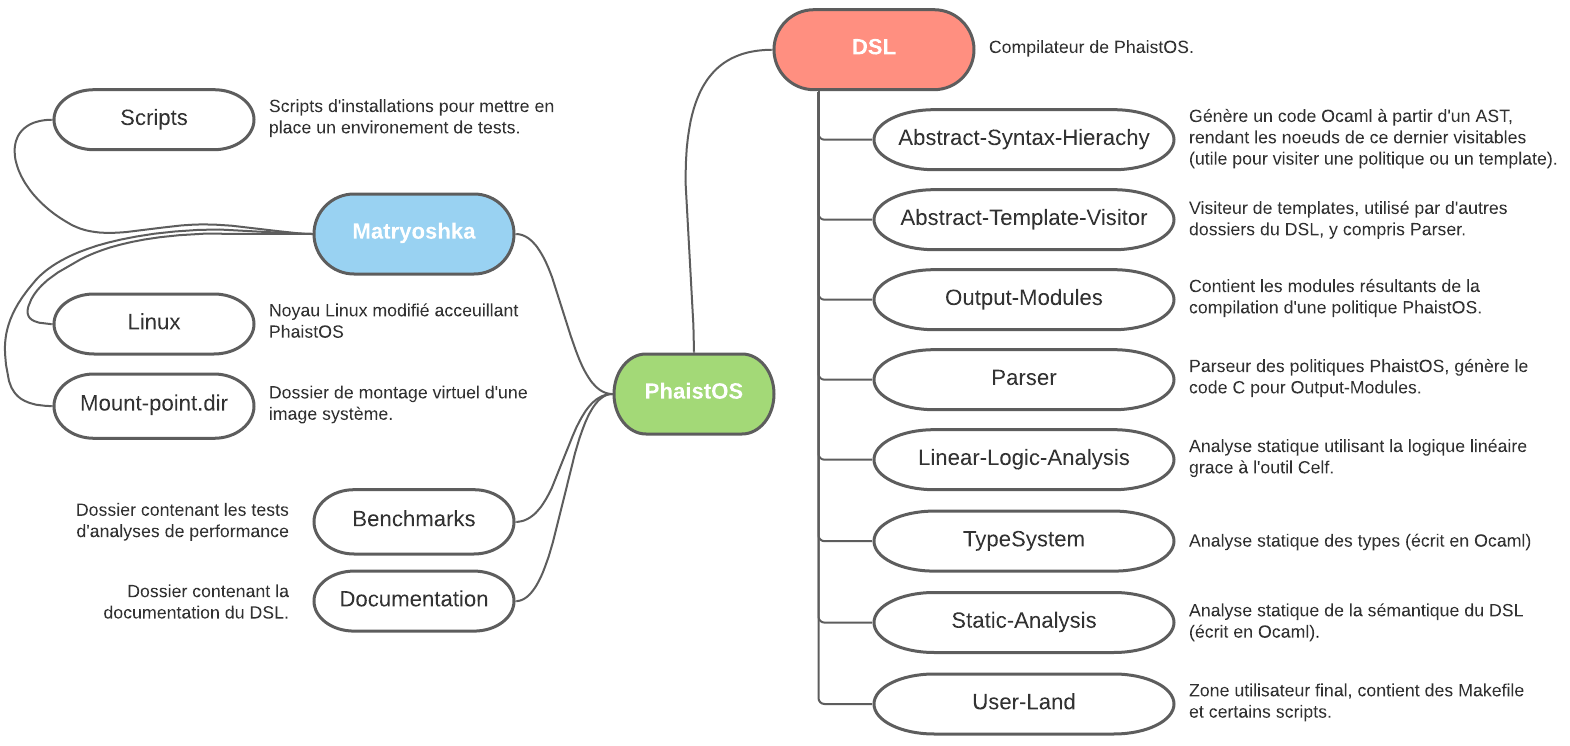
\includegraphics[width=12.5cm]{images/arch}
    \caption{Architecture du projet PhaistOS.}
    \label{fig:arch}
\end{figure}

Dans cette arborescence, on retrouve deux sections principales, et des sections 
secondaires. Concernant les sections principales, on retrouve évidemment le 
DSL, qui contiendra tous les outils nécessaires pour couvrir les objectifs de 
VeriAMOS, et on retrouvera aussi Matryoshka, qui permettra au prochain 
developpeur de mettre en place son environement de travail pour effectuer ses 
tests assez facilement. Les sections secondaires comprennent les tests de 
performances ainsi que la documentation générale, mais aussi d'autres moins 
significatives, qui n'ont pas été couvertes par mon stage (comme par exemple 
les fichiers de configuration Gitlab, ou les images Docker qu'avait mis en 
place Nick à l'époque).

\subsection{Fonctionnement du DSL}

Comme expliqué dans la Partie~\ref{why_phaistos}, PhaistOS possède un 
compilateur, un analyseur statique, et se base sur une politique écrite par un 
utilisateur final. Cette politique qui permettra de scripter le fonctionnement 
du planificateur d'E/S est écrite avec le langage du DSL PhaistOS.

\subsubsection{Le langage de PhaistOS}

<présenter le langage de PhaistOS>

\begin{table}[h!t]
    \centering
    \begin{tabular}{|l|l|} \hline
      \textbf{Event} & \textbf{Purpose} \\ \hline
      \texttt{INIT} & Initialisation de l'ordonnanceur \\
      \texttt{EXIT} & Nettoyage à la suppression de l'ordonnanceur \\
      \texttt{INSERT} & Enregistrement d'une nouvelle requête à traiter \\
      \texttt{REMOVE} & Suppression d'une requête en attente \\
      \texttt{DISPATCH} & Retourne la prochaine requête à envoyer pour le 
      disque \\
      \texttt{MERGE} & Procède à la fusion de deux requêtes \\
      \texttt{HAS\_WORK} & Indique s'il existe des requêtes en attente \\ \hline
    \end{tabular}
    \caption{List des événements PhaistOS}
    \label{tab:phaistos-events}
\end{table}

\subsubsection{l'outillage de PhaistOS}

<présenter l'architecture du compilateur>

<présenter les fichier .ast>

<présenter les templates>

\subsubsection{Vérification statique}

En réalité, comme on le voit sur la figure \ref{fig:arch}, il existe trois 
analyseurs : 
\begin{enumerate}
    \item Un analyseur sémantique de base, contenu dans \texttt{Static-Analysis}
    , écrit en Ocaml. Il permettra de vérifier l'arborescence et la sémantique 
    de la politique de l'utilisateur final. Pour cela il vérifie des règles de 
    bases, comme le parenthésage ou la présence de certains champs obligatoires.
    \item Un analyseur de type contenu dans \texttt{TypeSystem}, écrit en OCaml 
    et qui vient compléter l'analyseur précédent. Il vérifiera que les types 
    utilisés dans la politique écrite par l'utilisateur final sont corrects.
    \item Un vérificateur de propriétés de sécurité dans \texttt
    {Linear-Logic-Analysis}, concernant l'utilisation de l'API des requêtes d'E/
    S de Linux, à l'aide d'un outil externe, Celf~\cite{schack2008celf}.
\end{enumerate}
Mon stage n'a pas porté sur les analyseurs statiques, cependant les analyseurs 
écrits en Ocaml se rapproche de par leurs fonctionnement, au reste du DSL, j'ai 
donc pu travailler certains de leurs aspects.

% Pour comprendre le fonctionnement des analyseurs écrits en Ocaml, il faut 
% d'abord comprendre celui du DSL de manière générale.

\subsubsection{PhaistOS dans Linux}

<présenter son implémentation dans linux A MON ARRIVEE>

\subsection{Et ensuite ?}

<revenir sur les choses non-réalisées/complétées>

% L'analyseur en question est en réalité séparé en deux parties : une partie qui s'occupe de la vérifications des types et une autre pour exercer des vérifications spécifiques au domaine, qui utilise un système de preuve par logique linéaire.